\documentclass[11pt,a4paper]{article}
\usepackage[utf8]{inputenc}
\usepackage[T1]{fontenc}
\usepackage[english]{babel}
\usepackage[scaled=0.95]{helvet}
\renewcommand{\familydefault}{\sfdefault}
\usepackage[top=1.8cm,bottom=1.8cm,left=1.8cm,right=1.8cm]{geometry}
\usepackage{graphicx}
\usepackage{xcolor}
\usepackage{caption}
\usepackage{enumitem}
\usepackage{titlesec}
\usepackage{hyperref}
\graphicspath{{graphs/}}
\pagecolor{white}
\captionsetup{font=small,labelfont=bf}
\titleformat{\section}{\large\bfseries}{}{0pt}{}
\titlespacing*{\section}{0pt}{0.9em}{0.3em}
\setlength{\parindent}{0pt}
\setlength{\parskip}{0.45em}
\setlist[itemize]{leftmargin=1.2em,itemsep=0.15em,topsep=0.2em}
\pagestyle{plain}
% Text to be written once the results have been read
\newcommand{\tbc}[1]{\textcolor{red}{[TO BE COMPLETED: #1]}}
% Sample period written by Stata in graphs/smp_*.tex (n.a. if the file does not exist yet)
\newcommand{\smp}[1]{\IfFileExists{graphs/smp_#1.tex}{\input{graphs/smp_#1.tex}\unskip}{n.a.}}

\begin{document}

{\small POLICY NOTE \quad|\quad \tbc{authors, directorate} \quad|\quad \today}\par
\vspace{0.4em}
{\LARGE\bfseries Do energy price shocks feed into euro-area wages?}\par
\vspace{0.8em}

\textbf{Bottom line.} \tbc{one-sentence policy message on the pass-through of oil and gas
price shocks to negotiated and actual wages in the euro area}.

\section*{Main findings}

\begin{itemize}
\item \textbf{Negotiated wages.} \tbc{size, timing and persistence of the IV response of
  euro-area negotiated wages to a 10\% increase in oil and gas prices driven by supply
  shocks}.
\item \textbf{Actual hourly wages.} \tbc{IV response of gross wages per hour (national
  accounts) and comparison with negotiated wages, i.e.\ wage drift}.
\item \textbf{Oil versus gas.} \tbc{differences in the size and timing of the responses}.
\item \textbf{Countries.} \tbc{heterogeneity across Germany, France, Italy, Spain, the
  Netherlands and Belgium}.
\end{itemize}

\section*{Why it matters}

Whether energy-driven inflation spills over into wages is central to how persistent it
turns out to be. For consumer prices, Corsello and Foschi (2026) find that oil supply
shocks have short-lived effects, whereas gas supply shocks have stronger and more
persistent ones, and that indirect effects are muted when inflation is low but become
pronounced in high-inflation regimes. This note asks the same question for wages,
distinguishing negotiated wages, set in collective agreements, from actual wages per
hour worked.

\section*{How we estimate it}

We estimate local projections (Jordà, 2005) on quarterly data for the euro area and for
Germany, France, Italy, Spain, the Netherlands and Belgium, up to 12 quarters after the
shock. The quarter-on-quarter change in the spot price of oil (in US dollars) or of natural
gas (TTF) is instrumented with external supply shocks, as in Corsello and Foschi (2026): the
oil supply news shocks of Mori and Peersman for oil and the gas supply shocks of
Alessandri and Gazzani (2025) for gas (Stock and Watson, 2018). Responses are scaled to a
10\% increase in the price. The outcomes are
year-on-year growth in negotiated wages (ECB indicator) and in gross wages per hour
worked (Eurostat national accounts); HICP inflation, hours worked and the unemployment
rate are reported in the working document.

The shocks are monthly, the wage data quarterly: the instrument is the quarterly average
of the monthly shocks. Following Corsello and Foschi (2026), both stages control for two
lags of the outcome, of the price change, of log industrial production, of the
unemployment rate and of the 1-year Bund yield, and include a dummy for 2020--2022 and
its lags (Newey--West standard errors). The
strength of the instruments is checked with the effective $F$ statistic of Montiel Olea
and Pflueger (2013): \tbc{first-stage strength for oil and gas, euro area and countries}.
As robustness checks, the estimates are repeated with the three monthly shocks of each
quarter as separate instruments (Foroni, Marcellino and Schumacher, 2015), on pre-2020
data only and with smooth local projections (Barnichon and Brownlees, 2019);
reduced-form and OLS estimates are in the working document.
Euro-area sample for negotiated wages (shock dates): \smp{lp_iv_og_EA_contr}.

\section*{Discussion and policy implications}

\tbc{reading of the main IV results: size and timing of the response of negotiated and
actual hourly wages, compared with the pass-through to consumer prices}.

\textbf{Heterogeneity.} \tbc{oil versus gas and across countries (Figures 1 and 2)}.

\textbf{Robustness.} \tbc{monthly instruments, pre-COVID sample, smooth local
projections, reduced form and comparison with OLS}.

\textbf{Implications.} \tbc{what the results imply for the risk of second-round effects
from the current energy price shock}.

{\footnotesize
\textbf{References.} Alessandri and Gazzani (2025), \emph{Journal of Monetary Economics}
151, 103749; Barnichon and Brownlees (2019), \emph{Review of Economics and Statistics}
101(3); Corsello and Foschi (2026), Banca d'Italia, Questioni di Economia e Finanza
1024; Foroni, Marcellino and Schumacher (2015), \emph{Journal of the Royal Statistical
Society A} 178(1); Jordà (2005), \emph{American Economic Review} 95(1); Montiel Olea and
Pflueger (2013), \emph{Journal of Business and Economic Statistics} 31(3); Mori and
Peersman, ``Estimating the macroeconomic effects of oil supply news'', working paper;
Stock and Watson (2018), \emph{Economic Journal} 128(610).\par}

\begin{figure}[!htbp]
  \centering
  \caption{Response of negotiated wages to oil and gas price shocks}
  \label{fig:contr}
  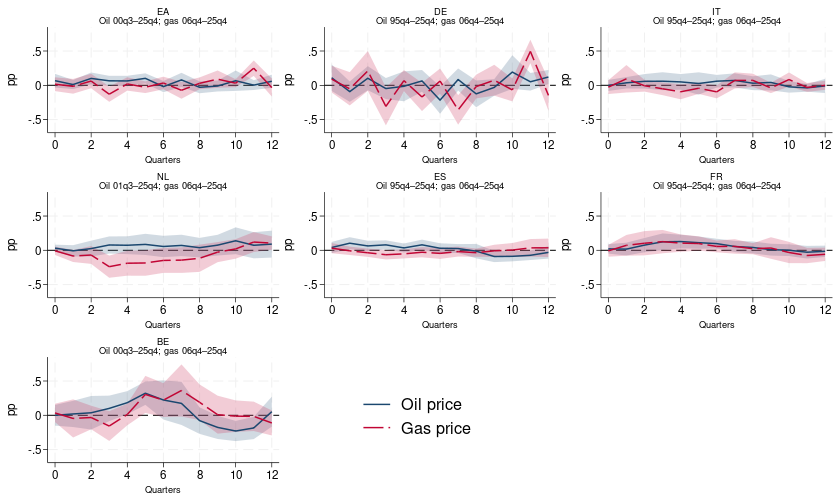
\includegraphics[width=0.72\textwidth]{lp_iv_og_ctry_contr.png}
  \begin{minipage}{\textwidth}\scriptsize
  \emph{Notes}: response (percentage points) of year-on-year growth in negotiated wages to a 10\%
  increase in the oil and natural gas prices;
  90\% confidence bands. IV local projections (oil: Mori--Peersman shocks; gas:
  Alessandri--Gazzani shocks; quarterly average of the monthly shocks as instrument). Time
  series for the euro area and for each country; same vertical
  scale in all panels; the sample (shock dates) for oil and gas is shown under each panel
  name.
  \end{minipage}

\end{figure}

\begin{figure}[!htbp]
  \centering
  \caption{Response of gross wages per hour worked to oil and gas price shocks}
  \label{fig:wageH}
  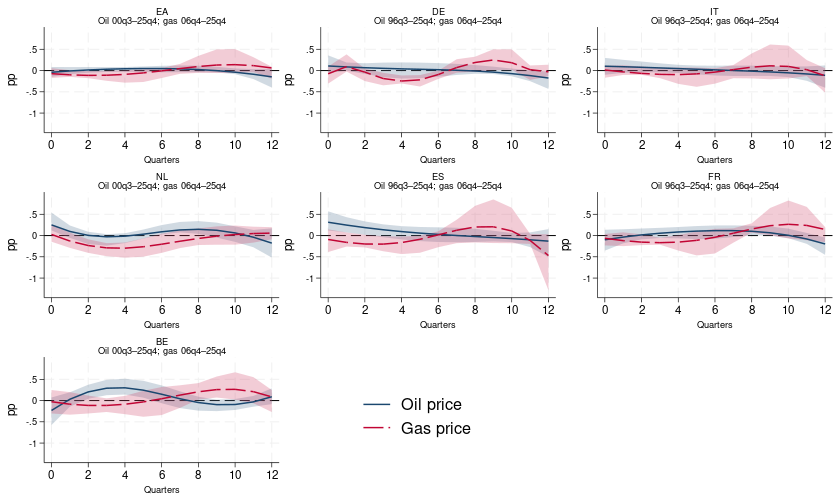
\includegraphics[width=0.72\textwidth]{lp_iv_og_ctry_wageH.png}
  \begin{minipage}{\textwidth}\scriptsize
  \emph{Notes}: see Figure 1.
  \end{minipage}
\end{figure}

\end{document}
